% Verification stages - coverage map: four checking stages hung off the
% artifacts they read, along a left-to-right artifact spine.
\documentclass[border=4pt]{standalone}
\usepackage{tikz}
\usetikzlibrary{arrows.meta, positioning, calc, fit, backgrounds}
\usepackage[T1]{fontenc}
\usepackage{lmodern}

% Ragged-right label text reads better in a figure without hyphen breaks.
\hyphenpenalty=10000
\exhyphenpenalty=10000

\definecolor{IHPfg}{RGB}{0,80,139}
\definecolor{IHPaccent}{RGB}{109,112,114}
\definecolor{IHPgreen}{RGB}{65,155,75}
\definecolor{IHPredsoft}{RGB}{210,80,80}
\definecolor{IHPamber}{RGB}{190,125,35}

\newcommand{\adkcard}[6]{%
    \node[adktitle, anchor=north] (#1t) at (#2) {#3};
    \node[adkrow=IHPgreen, anchor=north] (#1p) at ([yshift=-1.1mm]#1t.south)
        {{\bfseries proves}\, #4};
    \node[adkrow=IHPredsoft, anchor=north] (#1b) at ([yshift=-1.1mm]#1p.south)
        {{\bfseries blind to}\, #5};
    \if\relax\detokenize{#6}\relax
        \coordinate (#1n) at (#1b.south);
    \else
        \node[adknote, anchor=north] (#1n) at ([yshift=-1.1mm]#1b.south) {#6};
    \fi
    \begin{pgfonlayer}{background}
        \node[adkcardbox, fit=(#1t)(#1p)(#1b)(#1n)] (#1) {};
    \end{pgfonlayer}
}

\begin{document}
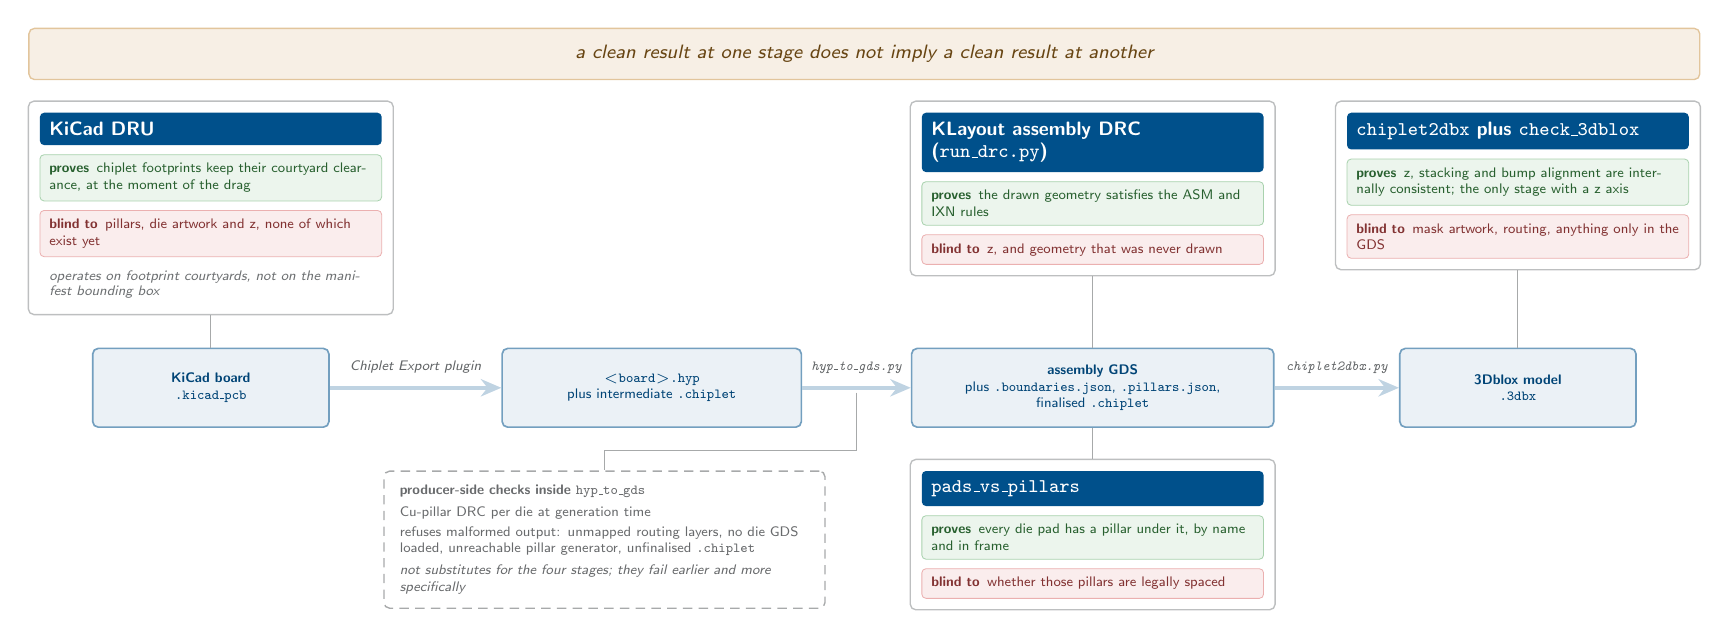
\begin{tikzpicture}[
    >=Stealth,
    adkart/.style={
        rectangle, rounded corners=2pt,
        draw=IHPfg!55, fill=IHPfg!8, line width=0.6pt,
        align=center, font=\sffamily\tiny, text=IHPfg!85!black,
        inner xsep=2mm, inner ysep=1.6mm, minimum height=10mm
    },
    adkcardbox/.style={
        rectangle, rounded corners=2pt,
        draw=IHPaccent!45, line width=0.5pt, inner sep=1.4mm
    },
    adktitle/.style={
        rectangle, rounded corners=1.5pt,
        fill=IHPfg, text=white, text width=41mm, align=left,
        inner xsep=1.2mm, inner ysep=1.2mm,
        font=\sffamily\scriptsize\bfseries
    },
    adkrow/.style={
        rectangle, rounded corners=1.5pt,
        fill=#1!10, draw=#1!45, line width=0.3pt,
        text width=41mm, align=left, inner xsep=1.2mm, inner ysep=1.1mm,
        font=\sffamily\tiny, text=#1!62!black
    },
    adknote/.style={
        text width=41mm, align=left, inner xsep=1.2mm, inner ysep=0.6mm,
        font=\sffamily\fontsize{4.6}{5.4}\selectfont\itshape, text=IHPaccent
    },
    adkprod/.style={
        rectangle, rounded corners=2pt,
        draw=IHPaccent!60, dash pattern=on 1.2mm off 0.8mm, line width=0.5pt,
        text width=52mm, align=left, inner xsep=2mm, inner ysep=1.8mm,
        font=\sffamily\tiny, text=IHPaccent!95!black
    },
    adkbanner/.style={
        rectangle, rounded corners=2pt,
        fill=IHPamber!12, draw=IHPamber!45, line width=0.5pt,
        minimum height=6.5mm, align=center,
        font=\sffamily\scriptsize\itshape, text=IHPamber!55!black
    },
    adkspine/.style={
        -{Stealth[length=2.6mm, width=2.2mm]},
        line width=1.6pt, color=IHPfg!25
    },
    adkleader/.style={line width=0.35pt, color=IHPaccent!60},
    adklbl/.style={
        font=\sffamily\fontsize{5}{6}\selectfont\itshape,
        text=IHPaccent!90!black
    }
]

% ---------- artifact spine ----------
\node[adkart, text width=26mm] (a1) at (0, 0)
    {\textbf{KiCad board}\\\texttt{.kicad\_pcb}};
\node[adkart, text width=34mm] (a2) at (5.6, 0)
    {\texttt{\textless board\textgreater.hyp}\\plus intermediate \texttt{.chiplet}};
\node[adkart, text width=42mm] (a3) at (11.2, 0)
    {\textbf{assembly GDS}\\plus \texttt{.boundaries.json},
     \texttt{.pillars.json},\\finalised \texttt{.chiplet}};
\node[adkart, text width=26mm] (a4) at (16.6, 0)
    {\textbf{3Dblox model}\\\texttt{.3dbx}};

\draw[adkspine] (a1) -- node[adklbl, above=0.4mm] {Chiplet Export plugin} (a2);
\draw[adkspine] (a2) -- node[adklbl, above=0.4mm] {\texttt{hyp\_to\_gds.py}} (a3);
\draw[adkspine] (a3) -- node[adklbl, above=0.4mm] {\texttt{chiplet2dbx.py}} (a4);

% ---------- stage cards above the spine ----------
\adkcard{c1}{0, 3.5}{KiCad DRU}
    {chiplet footprints keep their courtyard clearance, at the moment of the
     drag}
    {pillars, die artwork and z, none of which exist yet}
    {operates on footprint courtyards, not on the manifest bounding box}

\adkcard{c3}{11.2, 3.5}{KLayout assembly DRC (\texttt{run\_drc.py})}
    {the drawn geometry satisfies the ASM and IXN rules}
    {z, and geometry that was never drawn}
    {}

\adkcard{c2}{16.6, 3.5}{\texttt{chiplet2dbx} plus \texttt{check\_3dblox}}
    {z, stacking and bump alignment are internally consistent; the only stage
     with a z axis}
    {mask artwork, routing, anything only in the GDS}
    {}

\draw[adkleader] (c1.south) -- (a1.north);
\draw[adkleader] (c3.south) -- (a3.north);
\draw[adkleader] (c2.south) -- (a4.north);

% ---------- stage card below the spine ----------
\adkcard{c4}{11.2, -1.05}{\texttt{pads\_vs\_pillars}}
    {every die pad has a pillar under it, by name and in frame}
    {whether those pillars are legally spaced}
    {}

\draw[adkleader] (a3.south) -- (c4.north);

% ---------- producer-side checks ----------
\node[adkprod, anchor=north] (prod) at (5.0, -1.05)
    {{\bfseries producer-side checks inside \texttt{hyp\_to\_gds}}\\[0.6mm]
     Cu-pillar DRC per die at generation time\\[0.4mm]
     refuses malformed output: unmapped routing layers, no die GDS loaded,
     unreachable pillar generator, unfinalised \texttt{.chiplet}\\[0.7mm]
     {\fontsize{4.6}{5.4}\selectfont\itshape not substitutes for the four
      stages; they fail earlier and more specifically}};

\draw[adkleader] (8.2, -0.06) -- (8.2, -0.8) -| (prod.north);

% ---------- banner ----------
\node[fit=(c1)(c3)(c2), inner sep=0] (topbb) {};
\node[adkbanner, anchor=south, minimum width=212.2mm]
    at ([yshift=2.5mm]topbb.north)
    {a clean result at one stage does not imply a clean result at another};

\end{tikzpicture}
\end{document}
